\section[Method]{The method}
\sectionframe{03}{The method}{How are microstructures generated and steered toward properties?}{\faProjectDiagram}

% ------------------------------------------------------------------ data
\begin{frame}[source={Liao et al.\ (2026), Nat.\ Commun.\ 17, 11232, Methods}]{25 alloys, one map each}
  \begin{tikzpicture}[x=1mm,y=1mm]
    \useasboundingbox (0,0) rectangle (144,-54);
    % the orthogonal design: hot-rolling reduction across, annealing temperature down; each cell one alloy
    \node[anchor=south,label text] at (52,-2.4) {hot-rolling reduction at 900\,°C};
    \foreach \r [count=\c from 0] in {0,20,30,40,50}
      \node[anchor=south,small label,text=udsdark] at ({28+12*\c+6},-7.6) {\r\,\%};
    \foreach \t [count=\c from 0] in {650,750,850,950,1050}
      \node[anchor=east,small label,text=udsdark] at (27,{-8-7*\c-3.5}) {\t\,°C};
    \node[label text,rotate=90] at (5,-25.5) {annealing temperature};
    \foreach \r/\t/\h/\s/\sh in \alloygrid {
      \pgfmathtruncatemacro\c{\r==0 ? 0 : \r/10-1}
      \pgfmathtruncatemacro\w{(\t-650)/100}
      \fill[udsblue!\sh] ({28+12*\c},{-8-7*\w}) rectangle ++(12,-7);
      \ifnum\sh>40\def\tc{white}\else\def\tc{udsdark}\fi
      \node[font=\scriptsize,text=\tc,inner sep=0pt] at ({28+12*\c+6},{-8-7*\w-3.5}) {\h\,h};
    }
    \draw[white,line width=0.6pt] \foreach \c in {1,...,4} {({28+12*\c},-8) -- ++(0,-35)}
      \foreach \w in {1,...,4} {(28,{-8-7*\w}) -- ++(60,0)};
    \node[anchor=north west,small label,text width=62mm] at (28,-45.4)
      {each cell one alloy: its annealing time; darker: higher yield strength};
    % one alloy's data
    \fill[darktint] (96,-5.4) rectangle (144,-52);
    \cardhead{96}{0}{48}{udsdark}{Each alloy}
    \node[anchor=north west,inner sep=0pt] (map) at (98.5,-8)
      {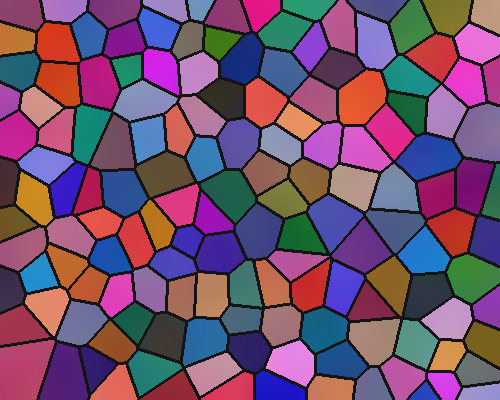
\includegraphics[width=20mm]{assets/drawn/grain-map-wide}};
    \node[anchor=north west,label text,text width=22mm] at (121,-8.4) {EBSD map\\ 1000\,×\,800 px\\ 0.5\,µm per px};
    \node[anchor=north west,label text,text width=42mm] at (98.5,-26.6)
      {colour: $(\varphi_1,\Phi,\varphi_2)\to$ red, green, blue};
    \begin{scope}[shift={(99.5,-48.5)}]
      \draw[udsgreymid,line width=0.5pt] (0,13) -- (0,0) -- (18,0);
      \draw[udsdark,line width=0.9pt] (0,0) -- (1.6,8.2) .. controls (4,10.2) and (12,11.6) .. (15.4,11.2)
        -- (16,8.8);
      \node[circle,fill=udsred,inner sep=0pt,minimum size=1.5mm] at (1.6,8.2) {};
      \node[circle,fill=udsred,inner sep=0pt,minimum size=1.5mm] at (16,8.8) {};
    \end{scope}
    \node[anchor=north west,label text,text width=22mm] at (121,-36.6) {tensile test:\\ yield strength,\\ elongation};
  \end{tikzpicture}
  \note{\textbf{11:30--12:40}\par
    The 25 alloys come from an orthogonal design: five hot-rolling reductions, five annealing
      temperatures and five annealing times, combined so that every pair of levels occurs once.\par
    Each cell is one alloy; the number is its annealing time and the shade its yield strength.\par
    More rolling and lower annealing temperatures give the stronger alloys.\par
    Each alloy has one EBSD map of 1000 by 800 pixels at 0.5 µm per pixel, a field of 500 by 400 µm,
      with the three Euler angles of each pixel stored as red, green and blue.\par
    Each alloy also has one yield strength and one elongation; how many tensile tests stand behind them
      is not stated.\par
    So the dataset is 25 maps and 25 pairs of property values.}
\end{frame}

% ----------------------------------------------------------------- split
\begin{frame}[source={Liao et al.\ (2026), Nat.\ Commun.\ 17, 11232, Results and Methods}]{Alloy split before cropping}
  \begin{tikzpicture}[x=1mm,y=1mm]
    \useasboundingbox (0,0) rectangle (144,-54);
    % stages, left to right
    \foreach \x/\t in {32/{EBSD maps},64/{patches, 100\,×\,100\,px},97/{+ flips, rotations},
        128/{+ degraded copies}}
      \node[anchor=north,label text,align=center] at (\x,0) {\t};
    \node[anchor=north,inner sep=0pt] (m1) at (32,-5.2) {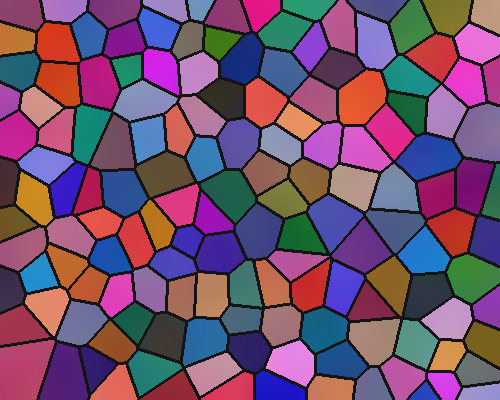
\includegraphics[width=16mm]{assets/drawn/grain-map-wide}};
    \node[anchor=north,inner sep=0pt] (m2) at (64,-5.2) {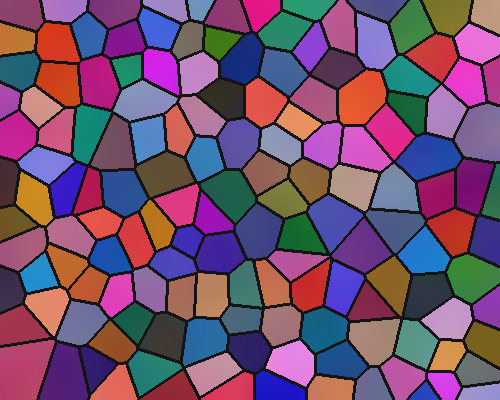
\includegraphics[width=16mm]{assets/drawn/grain-map-wide}};
    \draw[white,line width=0.35pt] \foreach \i in {1,...,9} {([xshift=\i*1.6mm]m2.north west) -- ([xshift=\i*1.6mm]m2.south west)}
      \foreach \j in {1,...,7} {([yshift=-\j*1.6mm]m2.north west) -- ([yshift=-\j*1.6mm]m2.north east)};
    \draw[udsred,line width=0.7pt] (m2.north west) rectangle ([xshift=1.6mm,yshift=-1.6mm]m2.north west);
    \node[inner sep=0pt] at (91.5,-9.7) {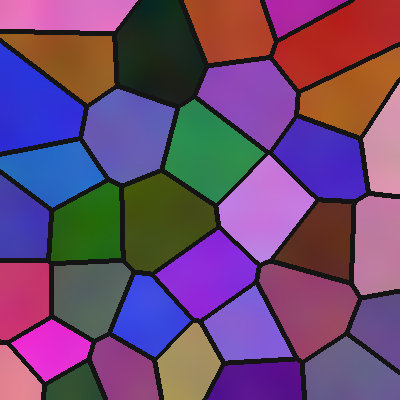
\includegraphics[width=9mm]{assets/drawn/grain-map}};
    \node[inner sep=0pt,rotate=90] at (102.5,-9.7) {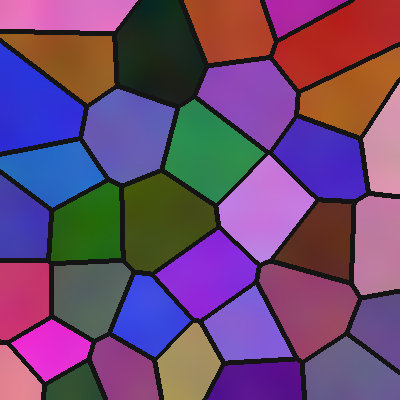
\includegraphics[width=9mm]{assets/drawn/grain-map}};
    \node[inner sep=0pt] at (122.5,-9.7) {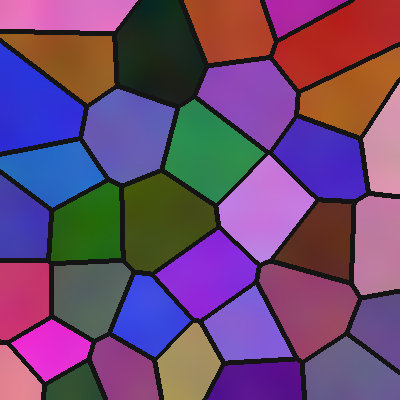
\includegraphics[width=9mm]{assets/drawn/grain-map}};
    \node[inner sep=0pt] at (133.5,-9.7) {
\includegraphics[width=9mm]{assets/drawn/grain-map-blurred}};
    % the two lanes
    \fill[bluetint] (0,-24) rectangle (144,-33.6);
    \fill[redtint] (0,-35.6) rectangle (144,-45.2);
    \node[anchor=west,label text,font=\footnotesize\bfseries,text=udsblue] at (1.6,-28.8) {training};
    \node[anchor=west,label text,font=\footnotesize\bfseries,text=udsred] at (1.6,-40.4) {test};
    \foreach \x/\ta/\tb in {32/{20 alloys}/{5 alloys},64/{1,600}/{400},97/{9,600}/{2,400},128/{57,600}/{14,400}} {
      \node[font=\small\bfseries,text=udsdark,inner sep=0pt] at (\x,-28.8) {\ta};
      \node[font=\small\bfseries,text=udsdark,inner sep=0pt] at (\x,-40.4) {\tb};}
    \foreach \x/\m in {48/\times 80,80.5/\times 6,112.5/\times 6} {
      \draw[flow,draw=udsgreymid] (\x-5,-28.8) -- (\x+5,-28.8);
      \draw[flow,draw=udsgreymid] (\x-5,-40.4) -- (\x+5,-40.4);
      \node[small label,anchor=south] at (\x,-23.4) {$\m$};}
    \goodstrip{-48.4}{test patches come from five alloys the model never sees in training}
  \end{tikzpicture}
  \note{\textbf{12:40--13:30}\par
    The split comes first: the 25 maps are divided at random into 20 training and 5 test alloys.\par
    Only then is each map cut into 80 patches of 100 by 100 pixels, 50 by 50 µm.\par
    Flips and rotations make six versions of each patch.\par
    Each version also gets five degraded copies (blur, distortion, black blocks, erosion and dilation),
      which the model learns to restore.\par
    That gives 72,000 images: 57,600 for training and 14,400 for testing.\par
    Because the split is by alloy, no test patch shares a map with a training patch: the same rule as
      splitting by specimen in segmentation.\par
    The images multiply; the alloys stay 25.}
\end{frame}

% ------------------------------------------------------------- generator
\begin{frame}[source={Liao et al.\ (2026), Nat.\ Commun.\ 17, 11232, Fig.\ 1a (CC BY-NC-ND 4.0) · Pandey et al.\ (2022), Trans.\ Mach.\ Learn.\ Res.}]
  {A VAE, refined by diffusion}
  \begin{tikzpicture}[x=1mm,y=1mm]
    \useasboundingbox (0,0) rectangle (144,-54);
    % Fig. 1a as published: its schematic, without the loss equation below it (pixel rows 0 to 258)
    \figpart{0}{0}{1}{0}{0}{2000}{258}{144}
    % the size of each part, under it; x from the part's pixel columns in the figure
    \tikzset{size/.style={anchor=north,small label,text=udsdark,align=center}}
    \node[size] at ({\fpx{113}},-19.8) {$100\times100$ px};
    \node[size,text=udsred] at ({\fpx{521}},-19.8) {128 numbers};
    \node[size] at ({\fpx{918}},-19.8) {$100\times100$ px};
    \node[size] at ({\fpx{1455}},-19.8) {one U-Net for every step};
    \node[size,anchor=north east] at (144,-19.8) {$100\times100$ px};
    % the two models, each under a bracket
    \draw[udsblue,line width=0.6pt] ({\fpx{40}},-23.6) -- ++(0,-1.4) -| ({\fpx{990}},-23.6);
    \node[anchor=north,label text,align=center,text width=68mm] at ({\fpx{515}},-26.4)
      {\textbf{variational autoencoder (VAE)}\\ three convolutional layers in, three transposed out\\
       loss $L_{\mathrm{pix}}+L_{\mathrm{edge}}+L_{\mathrm{SSIM}}+L_{\mathrm{KL}}$};
    \draw[udsblue,line width=0.6pt] ({\fpx{1148}},-23.6) -- ++(0,-1.4) -| ({\fpx{1997}},-23.6);
    \node[anchor=north,label text,align=center,text width=60mm] at ({\fpx{1572}},-26.4)
      {\textbf{conditional diffusion model (DDPM)}\\ a U-Net predicts the noise, guided by $x_V$\\
       loss: the same three terms on the noise};
    % how the generator is trained, and how it generates
    \foreach \i/\c/\icon/\h/\b in {
        0/udsblue/\faImages/training data/{57,600 images of the 20 training alloys: patches to reproduce,
          and degraded copies to restore},
        1/udsred/\faStar/generation/{a code from the search goes through the decoder, then the diffusion
          model: a new patch}} {
      \fill[\c!8] ({\i*74},-39) rectangle ++(70,-14.6);
      \fill[\c] ({\i*74},-39) rectangle ++(1.2,-14.6);
      \node[anchor=north west,inner sep=0pt,font=\scriptsize\bfseries,text=\c] at ({\i*74+3.4},-40.8)
        {\icon\enspace\h};
      \node[anchor=north west,inner sep=0pt,font=\scriptsize,text=udsdark,text width=64.6mm,align=left,
        execute at begin node={\hyphenpenalty=10000\raggedright}] at ({\i*74+3.4},-44.8) {\b};}
  \end{tikzpicture}
  \note{\textbf{13:30--14:20}\par
    This is the paper's own diagram of its generator, Fig.~1a.\par
    The VAE compresses each patch of 100 by 100 pixels into a code z of 128 numbers and decodes it into
      $x_V$, which is smooth.\par
    A conditional diffusion model then refines $x_V$: its U-Net predicts the noise step by step and sees
      $x_V$ at every step, the pairing of DiffuseVAE; the red arrow marks that condition.\par
    Both models are trained with the pixel, edge and SSIM terms of the next slide: the VAE on its output,
      the diffusion model on the noise it predicts.\par
    Training uses the 57,600 images of the 20 training alloys, with Adam over 100 epochs.\par
    The code z is what the search moves around later.}
\end{frame}

% ------------------------------------------------------------------ loss
\begin{frame}[source={Liao et al.\ (2026), Nat.\ Commun.\ 17, 11232, Eqs.\ 1--9 · Sobel and Feldman (1968), Stanford AI Project · Wang et al.\ (2004), IEEE Trans.\ Image Process.\ 13, 600}]{Optimization Loss}
  \begin{tikzpicture}[x=1mm,y=1mm]
    \useasboundingbox (0,0) rectangle (144,-54);
    % the equation, each term above its column
    \foreach \x/\t in {5/{L\;=},22/{L_{\mathrm{pix}}},47/{+},72/{\color{udsblue}L_{\mathrm{edge}}},97/{+},
        122/{\color{udsblue}L_{\mathrm{SSIM}}}}
      \node[font=\LARGE,text=udsdark,inner sep=0pt] at (\x,-3.2) {$\t$};
    \foreach \x/\c/\h in {0/udsgreymid/{pixel values},50/udsblue/{edges},100/udsblue/{structure}} {
      \fill[\c!8] (\x,-16.6) rectangle ++(44,-35.4);
      \cardhead{\x}{-11.2}{44}{\c}{\h}}
    % pixel values
    \node[anchor=north,font=\small,text=udsdark,inner sep=0pt] at (22,-19.6)
      {$\displaystyle\frac{1}{n}\sum_{i=1}^{n}|x_i-\hat{x}_i|$};
    \node[anchor=north west,card text,text width=40mm] at (2,-31)
      {Mean Absolute\\ Difference (MAE)\\[0.8mm] every pixel weighs the same; boundaries are few pixels};
    % edges
    \node[anchor=north,font=\small,text=udsdark,inner sep=0pt] at (72,-19.6)
      {$\mathrm{mean}\,|S\ast x-S\ast\hat{x}|$};
    \node[anchor=north west,inner sep=0pt] (e1) at (54,-25.4) {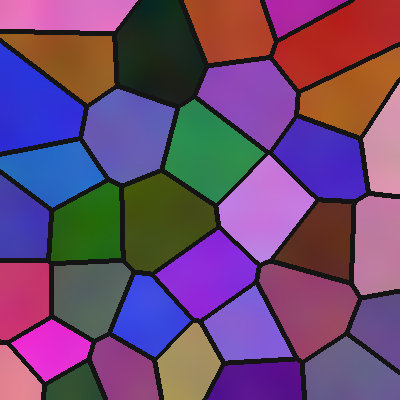
\includegraphics[width=12mm]{assets/drawn/grain-map}};
    \node[anchor=north west,inner sep=0pt] (e2) at (78,-25.4) {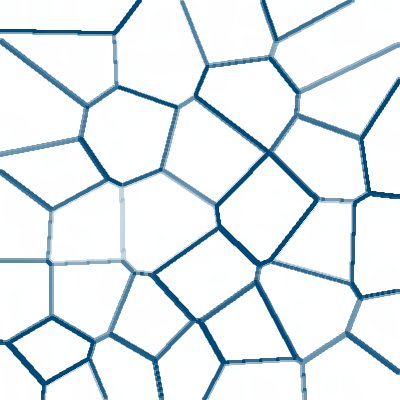
\includegraphics[width=12mm]{assets/drawn/grain-map-edges}};
    \draw[icon frame,udsgreylight] (e2.south west) rectangle (e2.north east);
    \draw[flow,draw=udsblue] (e1.east) -- node[above=0.6mm,small label,text=udsblue] {$S\ast$} (e2.west);
    \node[anchor=north west,card text,text width=40mm] at (52,-40)
      {Sobel filter $S$, across and down: large at grain boundaries};
    % structure
    \node[anchor=north,font=\small,text=udsdark,inner sep=0pt] at (122,-19.6)
      {$1-\mathrm{SSIM}(x,\hat{x})$};
    \node[anchor=north west,inner sep=0pt] (s1) at (104,-25.4) {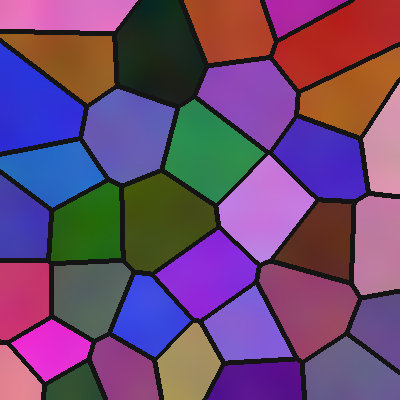
\includegraphics[width=12mm]{assets/drawn/grain-map}};
    \node[anchor=north west,inner sep=0pt] (s2) at (128,-25.4) {
\includegraphics[width=12mm]{assets/drawn/grain-map-blurred}};
    \node[small label,text=udsblue] at (122,-31.4) {$x$ vs $\hat{x}$};
    \node[anchor=north west,card text,text width=40mm] at (102,-40)
      {means, contrasts and correlation: orientation inside grains};
  \end{tikzpicture}
  \note{\textbf{14:20--15:30}\par
    The loss is the sum of three terms, added without weights.\par
    The pixel term is the mean absolute difference between original and reconstruction; boundaries
      cover few pixels, so it hardly sees them.\par
    The edge term applies the Sobel filter, a three-by-three derivative filter from Sobel and Feldman,
      1968, across and down both images and compares the responses: it is large where colours change,
      at grain boundaries.\par
    The structure term is one minus the structural similarity index (SSIM) of Wang and colleagues, 2004,
      which compares the means, contrasts and correlation of the two images; the authors use it for the
      orientation inside and between grains.\par
    The VAE adds its Kullback--Leibler term; the diffusion model applies the same three terms to the
      noise it predicts.\par
    All three compare colours, that is, Euler angles read as intensities.}
\end{frame}

% ------------------------------------------------------------------ SSIM
\begin{frame}[source={Liao et al.\ (2026), Nat.\ Commun.\ 17, 11232, Eqs.\ 4--9 · Wang et al.\ (2004), IEEE Trans.\ Image Process.\ 13, 600}]{Structural Similarity (SSIM)}
  \begin{tikzpicture}[x=1mm,y=1mm]
    \useasboundingbox (0,0) rectangle (144,-54);
    \tikzset{pair image/.style={anchor=north west,inner sep=0pt},
      component value/.style={anchor=north,inner sep=0pt,font=\scriptsize,text=udsdark},
      component formula/.style={anchor=north,inner sep=0pt,font=\footnotesize,text=udsdark},
      component meaning/.style={anchor=north,inner sep=0pt,font=\scriptsize,text=udsdark}}
    % three components; each compares the patch with a copy that changes only what it measures
    \foreach \i/\h in {0/{luminance $L$},1/{contrast $C$},2/{structure $S$}} {
      \fill[bluetint] ({\i*49},-5.4) rectangle ++(46,-29.4);
      \cardhead{\i*49}{0}{46}{udsblue}{\h}
      \node[pair image] at ({\i*49+7.4},-7.4) {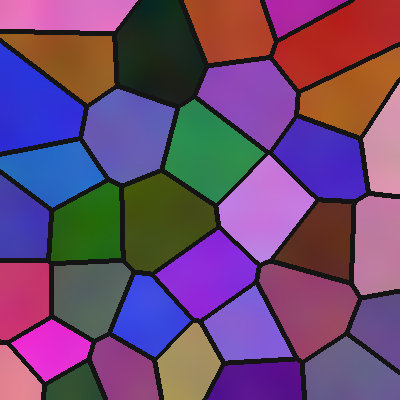
\includegraphics[width=11mm]{assets/drawn/grain-map}};
      \node[small label,text=udsdark] at ({\i*49+23},-12.9) {vs};}
    \node[pair image] at (28.6,-7.4) {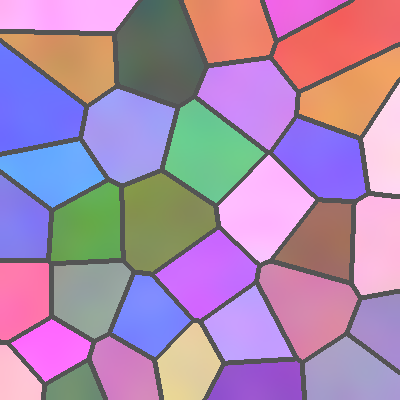
\includegraphics[width=11mm]{assets/drawn/ssim-bright}};
    \node[pair image] at (77.6,-7.4) {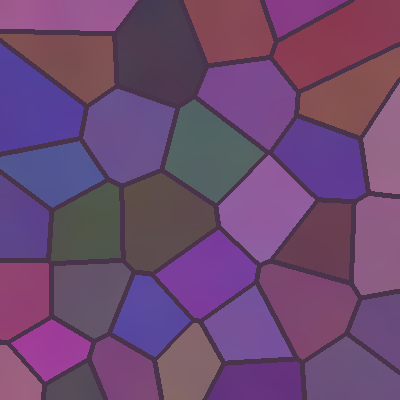
\includegraphics[width=11mm]{assets/drawn/ssim-flat}};
    \node[pair image] at (126.6,-7.4) {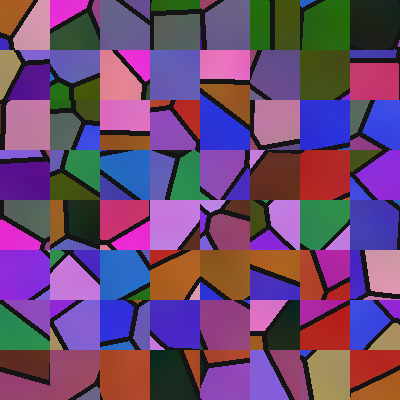
\includegraphics[width=11mm]{assets/drawn/ssim-shuffled}};
    \node[component value] at (23,-19.6)
      {\textcolor{udsred}{$L=\ssimBrightL$}\enspace $C=\ssimBrightC$\enspace $S=\ssimBrightS$};
    \node[component value] at (72,-19.6)
      {$L=\ssimFlatL$\enspace \textcolor{udsred}{$C=\ssimFlatC$}\enspace $S=\ssimFlatS$};
    \node[component value] at (121,-19.6)
      {$L=\ssimShuffledL$\enspace $C=\ssimShuffledC$\enspace \textcolor{udsred}{$S=\ssimShuffledS$}};
    \node[component formula] at (23,-23.2) {$\dfrac{2\mu_x\mu_{\hat x}+C_1}{\mu_x^2+\mu_{\hat x}^2+C_1}$};
    \node[component formula] at (72,-23.2) {$\dfrac{2\sigma_x\sigma_{\hat x}+C_2}{\sigma_x^2+\sigma_{\hat x}^2+C_2}$};
    \node[component formula] at (121,-23.2) {$\dfrac{\sigma_{x\hat x}+C_3}{\sigma_x\sigma_{\hat x}+C_3}$};
    \node[component meaning] at (23,-31) {brightness: the means $\mu$};
    \node[component meaning] at (72,-31) {contrast: the spreads $\sigma$};
    \node[component meaning] at (121,-31) {pattern: the covariance $\sigma_{x\hat x}$};
    % multiplied as the paper does, and turned into a loss
    \fill[bluetint] (0,-37.6) rectangle (144,-53.6);
    \node[anchor=west,inner sep=0pt,font=\footnotesize,text=udsdark] at (2.4,-42.6)
      {$\mathrm{SSIM}=L^{\alpha}\,C^{\beta}\,S^{\gamma}$};
    \node[anchor=west,small label,text=udsdark,text width=44mm] at (2.4,-48.8)
      {paper: $\alpha=\beta=\gamma=1$, $C_3=C_2/2$};
    \node[anchor=west,inner sep=0pt,font=\footnotesize,text=udsdark] (eq8) at (46.6,-45.6)
      {$=\dfrac{(2\mu_x\mu_{\hat x}+C_1)(2\sigma_{x\hat x}+C_2)}{(\mu_x^2+\mu_{\hat x}^2+C_1)(\sigma_x^2+\sigma_{\hat x}^2+C_2)}$};
    \draw[flow,draw=udsblue] ([xshift=1.6mm]eq8.east) -- ++(5.4,0);
    \node[anchor=west,inner sep=0pt,font=\footnotesize,text=udsdark] (loss) at ([xshift=8.6mm]eq8.east)
      {$L_{\mathrm{SSIM}}=1-\mathrm{SSIM}$};
    \node[anchor=north west,small label,text=udsdark] at ([yshift=-1.4mm]loss.south west) {zero for identical patches};
  \end{tikzpicture}
  \note{\textbf{15:30--16:40}\par
    SSIM compares two patches in three ways, each through one statistic of the pixel values.\par
    Luminance compares the means: a brighter copy of the patch scores $L=\ssimBrightL$, while $C$ and $S$
      stay near 1.\par
    Contrast compares the standard deviations: a flattened copy scores $C=\ssimFlatC$.\par
    Structure compares the patterns through the covariance: shuffling the patch's tiles keeps its mean
      and spread but drops $S$ to \ssimShuffledS.\par
    The product, with all exponents 1 and $C_3=C_2/2$ as in the paper, gives its Eq.~8; the loss is one
      minus SSIM.\par
    The brighter copy differs by \ssimBrightM{} per pixel on average and keeps SSIM \ssimBrightQ; the blurred
      patch of slide 4 differs by only \ssimBlurredM{} but drops to \ssimBlurredQ: SSIM sees lost structure
      that a pixel loss barely notices.}
\end{frame}

% --------------------------------------------------- failure case, fixed
\begin{frame}[source={Liao et al.\ (2026), Nat.\ Commun.\ 17, 11232, Fig.\ 2c (CC BY-NC-ND 4.0)}]
  {The same patches, with the new loss}
  \begin{tikzpicture}[x=1mm,y=1mm]
    \useasboundingbox (0,0) rectangle (144,-54);
    \figpart{36}{0}{2}{340}{770}{1897}{1537}{104}
    \node[anchor=east,label text,align=right] at (33,{\fpy{884}}) {real patches};
    \node[anchor=east,label text,align=right,text=udsred] at (33,{\fpy{1155}}) {pixel loss only};
    \node[anchor=east,label text,align=right,text=testgreen] at (33,{\fpy{1423}}) {with edge and\\SSIM terms};
  \end{tikzpicture}
  \note{\textbf{16:40--17:20}\par
    The same six test patches, with a third row: the model trained with all three terms.\par
    The boundaries are sharp again, and each grain has nearly one colour.\par
    The pixel loss itself also falls, from about 0.20 to about 0.10 according to the text; the plotted
      curve settles nearer 0.07.\par
    Two more reconstruction terms also weaken the Kullback--Leibler term relative to the rest, which by
      itself can lower a VAE's reconstruction error; the paper does not separate the two effects.\par
    The comparison with a standard VAE, a Wasserstein GAN and a standard DDPM is only in the
      Supplementary Information.}
\end{frame}

% ------------------------------------------------------------ descriptor
\begin{frame}[source={Liao et al.\ (2026), Nat.\ Commun.\ 17, 11232, after Fig.\ 4a and Methods · Pearson (1901), Philos.\ Mag.\ 2, 559}]{Six numbers per alloy}
  \begin{tikzpicture}[x=1mm,y=1mm]
    \useasboundingbox (0,0) rectangle (144,-54);
    \tikzset{dims/.style={anchor=north,small label,text=udsdark,align=center},
      op/.style={small label,text=udsgrey,align=center},
      back/.style={anchor=north,small label,text=udsred,align=center}}
    % one alloy's map, cut into 10 x 8 patches of 100 x 100 pixels
    \node[anchor=north west,inner sep=0pt] at (0,0) {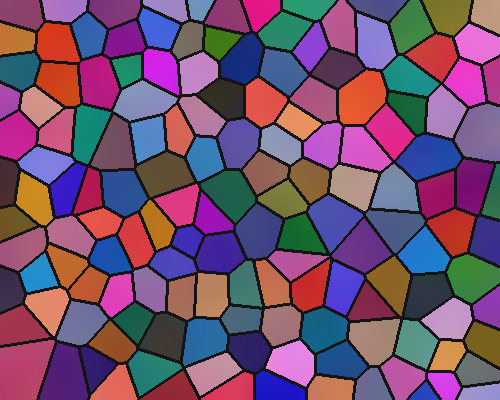
\includegraphics[width=25mm]{assets/drawn/grain-map-wide}};
    \draw[white,line width=0.35pt] \foreach \i in {1,...,9} {(\i*2.5,0) -- (\i*2.5,-20)}
      \foreach \j in {1,...,7} {(0,-\j*2.5) -- (25,-\j*2.5)};
    \node[dims] at (12.5,-20.8) {one alloy, $1000\times800$ px:\\ 80 patches};
    % the encoder gives one code of 128 numbers per patch
    \draw[flow] (25.6,-10) -- (28.2,-10);
    \filldraw[fill=bluetint,draw=udsblue,line width=0.5pt] (28.8,-3.4) -- (36.4,-6.8) -- (36.4,-13.2) -- (28.8,-16.6) -- cycle;
    \node[label text,rotate=90,font=\scriptsize] at (32.4,-10) {encoder};
    \draw[flow] (37,-10) -- (39.6,-10);
    \codematrix{40.2}{-1}{16}{18}{1}
    \node[dims] at (48.2,-20.8) {80 codes\\ $\times$ 128 numbers};
    % mean and spread over the 80 patches
    \draw[flow] (56.8,-7.2) -- node[above=0.4mm,op,sloped] {mean} (65.4,-5.4);
    \draw[flow] (56.8,-12.8) -- node[below=0.4mm,op,sloped] {spread} (65.4,-14.6);
    \pgfmathsetseed{80}
    \foreach \c in {0,...,15} {
      \pgfmathtruncatemacro\shadeA{20+50*rnd}
      \pgfmathtruncatemacro\shadeB{10+45*rnd}
      \filldraw[fill=udsblue!\shadeA,draw=udsblue,line width=0.3pt] ({66+1.25*\c},-4.2) rectangle ++(1.25,-2.4);
      \filldraw[fill=udsdark!\shadeB,draw=udsdark,line width=0.3pt] ({66+1.25*\c},-13.4) rectangle ++(1.25,-2.4);}
    \node[anchor=south,small label,text=udsdark] at (76,-3.6) {$\mu$: 128 numbers};
    \node[dims] at (76,-16.4) {$\sigma$: 128 numbers};
    % PCA, fitted on the 25 alloys: the first three components of each
    \draw[flow] (86.6,-5.4) -- node[above=0.4mm,op] {PCA} (92.4,-5.4);
    \draw[flow] (86.6,-14.6) -- node[below=0.4mm,op] {PCA} (92.4,-14.6);
    \foreach \j in {0,1,2} {
      \filldraw[fill=bluetint,draw=udsblue,line width=0.5pt] ({93+2.4*\j},-4.2) rectangle ++(2.4,-2.4);
      \filldraw[fill=darktint,draw=udsdark,line width=0.5pt] ({93+2.4*\j},-13.4) rectangle ++(2.4,-2.4);}
    \node[op,anchor=north] at (96.6,-19.6) {first 3 of\\ 24 components};
    % the descriptor
    \draw[flow] (100.8,-5.4) to[out=0,in=180] (107.4,-9.4);
    \draw[flow] (100.8,-14.6) to[out=0,in=180] (107.4,-10.6);
    \descstrip{108}{-8.8}{2.4}{2.4}
    \node[anchor=south,small label,text=udsdark] at (115.2,-8.2) {descriptor};
    \node[anchor=west,small label,text=udsdark] at (123.2,-10) {6 numbers};
    % the table it fills: one row per alloy, beside the measured properties
    \draw[flow] (115.2,-11.6) -- (115.2,-31.8);
    \descstrip{108}{-32.4}{2.4}{3}
    \foreach \x/\l in {122.4/YS,129.4/El}
      \node[draw=udsgreymid,fill=darktint,line width=0.3pt,minimum width=7mm,minimum height=3mm,inner sep=0pt,
        anchor=north west,font=\scriptsize,text=udsdark] at (\x,-32.4) {\l};
    \foreach \r in {1,...,3} \foreach \x/\w in {108/14.4,122.4/7,129.4/7}
      \draw[udsgreylight,line width=0.3pt,fill=white] (\x,{-32.4-3*\r}) rectangle ++(\w,-3);
    \node[small label,text=udsdark] at (122.4,-45.4) {$\vdots$};
    \node[dims,text width=36mm] at (122.4,-48.9) {25 alloys: six numbers, yield strength, elongation};
    % the way back, which the search uses: below the labels, up to the map's label at the end
    \draw[udsred,line width=0.6pt,dash pattern=on 1.6pt off 1.2pt,-{Stealth[length=1.6mm,width=1.2mm]}]
      (109.2,-11.6) -- (109.2,-31) -- (12.5,-31) -- (12.5,-27.6);
    \foreach \x/\l in {96.6/inverse PCA,76/{$\mu$, $\sigma$},48.2/draw 80 codes,32.6/decode}
      \node[back] at (\x,-31.8) {\l};
    \node[anchor=north west,small label,text=udsred,text width=92mm] at (0,-36.4)
      {the way back, for the search: six numbers give a mean and a spread, 80 codes are drawn from them and
       decoded into new patches};
  \end{tikzpicture}
  \note{\textbf{17:20--18:10}\par
    To link microstructures with properties, each alloy needs one descriptor.\par
    The 80 patches of its map are encoded, which gives 80 codes of 128 numbers.\par
    Their mean and standard deviation over the patches describe the alloy: what its patches look like
      on average, and how much they vary.\par
    Principal component analysis (PCA, Pearson 1901), fitted on the 25 alloys, keeps the first three of
      24 components of each, so every alloy becomes six numbers beside its measured properties.\par
    PCA can be inverted, the red path: six numbers map back to a mean and a spread, from which new codes
      are drawn and decoded.\par
    The number of components was chosen by the fidelity of the generated patches (Supplementary
      Information).}
\end{frame}

% ---------------------------------------------------------------- search
\begin{frame}[source={Liao et al.\ (2026), Nat.\ Commun.\ 17, 11232, after Fig.\ 4a · Deb et al.\ (2002), IEEE Trans.\ Evol.\ Comput.\ 6, 182}]{A genetic search in six numbers}
  \begin{tikzpicture}[x=1mm,y=1mm]
    \useasboundingbox (0,0) rectangle (144,-54);
    \tikzset{glyph label/.style={anchor=north,small label,text=udsdark,align=center},
      op/.style={anchor=south,small label,text=udsgrey,align=center,yshift=1mm}}
    % the loop: four steps on cards, run for 500 generations
    \foreach \i/\h in {0/population,1/predict,2/keep the best,3/{cross over, mutate}} {
      \pgfmathsetmacro\cx{\i*38}
      \fill[bluetint] (\cx,-5.4) rectangle ++(30,-13.4);
      \cardhead{\cx}{0}{30}{udsblue}{\h}}
    \foreach \i in {0,1,2} \draw[flow,draw=udsblue] ({\i*38+30.4},-12.1) -- ({\i*38+37.6},-12.1);
    % population: 10 descriptors of six numbers
    \foreach \k in {0,...,4} {\descstrip{4}{-7-1.7*\k}{1.5}{1.2}\descstrip{17}{-7-1.7*\k}{1.5}{1.2}}
    \node[glyph label] at (15,-15.6) {10 descriptors};
    % predict: one tree model per property
    \minitree{45.5}{-7.2}
    \minitree{60.5}{-7.2}
    \node[glyph label] at (45.5,-14.2) {strength};
    \node[glyph label] at (60.5,-14.2) {elongation};
    % keep the best: fronts and crowding, as on slide 10
    \begin{scope}[shift={(80.5,-17.4)}]
      \draw[udsgreymid,line width=0.4pt] (0,10.4) -- (0,0) -- (22,0);
      \begin{scope}[x=22mm,y=10mm]
        \drawfronttwo[udsgreymid,line width=0.5pt,dash pattern=on 1.2pt off 0.9pt]
        \drawfrontone[udsblue,line width=0.7pt]
        \foreach \x/\y/\r in \paretopoints {
          \ifcase\r\or\def\rc{udsblue}\or\def\rc{udsgreymid}\else\def\rc{udsgreylight}\fi
          \node[circle,fill=\rc,inner sep=0pt,minimum size=1.2mm] at (\x,\y) {};}
      \end{scope}
    \end{scope}
    % cross over and mutate: a child from two parents, one number changed
    \foreach \j in {0,...,5} {
      \filldraw[fill=udsblue!20,draw=udsblue,line width=0.3pt] ({116.6+1.8*\j},-7.4) rectangle ++(1.8,-1.8);
      \filldraw[fill=udsblue!65,draw=udsblue,line width=0.3pt] ({116.6+1.8*\j},-10.4) rectangle ++(1.8,-1.8);
      \ifnum\j<3\def\cf{udsblue!20}\else\def\cf{udsblue!65}\fi
      \ifnum\j=4\def\cf{udsred!70}\fi
      \filldraw[fill=\cf,draw=udsblue,line width=0.3pt] ({131.4+1.8*\j},-8.9) rectangle ++(1.8,-1.8);}
    \draw[flow,draw=udsblue,line width=0.5pt] (128.4,-9.8) -- (130.8,-9.8);
    \node[glyph label] at (122,-13.4) {parents};
    \node[glyph label] at (136.8,-13.4) {child, one\\ number mutated};
    % 500 generations: the way round
    \draw[flow,draw=udsblue] (129,-18.8) -- (129,-21.8) -- (15,-21.8) -- (15,-19.2);
    \node[fill=white,inner sep=1mm,font=\footnotesize\bfseries,text=udsblue] at (72,-21.8) {500 generations};
    % the way back to microstructures, for the 5 best
    \draw[flow] (5,-18.8) -- (5,-30.8);
    \node[anchor=west,small label,text=udsdark] at (6.4,-25) {the 5 best};
    \foreach \k in {0,...,4} \descstrip{0}{-31.4-1.8*\k}{1.8}{1.3}
    \node[glyph label] at (5.4,-41.6) {5 descriptors};
    \draw[flow] (12.2,-36) -- node[op] {inverse\\ PCA} (26.4,-36);
    \pgfmathsetseed{80}
    \foreach \c in {0,...,15} {
      \pgfmathtruncatemacro\shadeA{20+50*rnd}
      \pgfmathtruncatemacro\shadeB{10+45*rnd}
      \filldraw[fill=udsblue!\shadeA,draw=udsblue,line width=0.3pt] ({27.2+1.25*\c},-32.6) rectangle ++(1.25,-2.4);
      \filldraw[fill=udsdark!\shadeB,draw=udsdark,line width=0.3pt] ({27.2+1.25*\c},-37) rectangle ++(1.25,-2.4);}
    \node[glyph label] at (37.2,-40.2) {$\mu$, $\sigma$: 128 each};
    \draw[flow] (48,-36) -- node[op] {draw\\ 80 codes} (62.2,-36);
    \codematrix{63}{-30.6}{12}{11}{1}
    \node[glyph label] at (69,-42.4) {80 codes};
    \draw[flow] (75.8,-36) -- node[op] {decode,\\ refine} (90,-36);
    \node[anchor=north west,inner sep=0pt] at (90.8,-29.6) {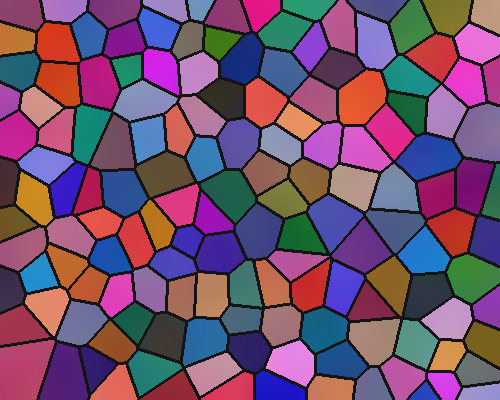
\includegraphics[width=25mm]{assets/drawn/grain-map-wide}};
    \draw[white,line width=0.35pt] \foreach \i in {1,...,9} {(90.8+\i*2.5,-29.6) -- (90.8+\i*2.5,-49.6)}
      \foreach \j in {1,...,7} {(90.8,-29.6-\j*2.5) -- (115.8,-29.6-\j*2.5)};
    \node[glyph label] at (103.3,-50.2) {80 new patches};
    \node[text=udsred,font=\small] at (120.2,-34.4) {\faStar};
    \node[anchor=north west,label text,text width=21mm,text=udsred] at (122.6,-32.4)
      {a proposed microstructure for each descriptor};
  \end{tikzpicture}
  \note{\textbf{18:10--19:00}\par
    The loop of section 2, run on the six numbers.\par
    Two gradient-boosted tree models, one per property, fitted on the 20 training alloys, predict yield
      strength and elongation from a descriptor; they are the objectives.\par
    NSGA-II evolves a population of 10 descriptors over 500 generations; the paper's average hypervolume
      improvement, the area the candidates span above the weakest measured alloy, levels off after about
      150 generations.\par
    The five best final descriptors go back through the inverse PCA to a mean and a spread; 80 codes are
      drawn from them and decoded into patches, the proposed microstructures.}
\end{frame}
